
\section[HybridSim]{Гибридная метрика семантической близости}

\subsection{}

\begin{frame}
\frametitle{Публикациии}
\begin{itemize}
\item Panchenko A., Morozova O. \textbf{A Study of Hybrid Similarity Measures
for Semantic Relation Extraction.} // Innovative Hybrid Approaches to the Processing of Textual Data Workshop, EACL 2012 — Avignon (France), 2012 — pp. 10–18 
\item Panchenko A., \textbf{Similarity Measures for Semantic Relation
Extraction.} PhD thesis. Universit\'{e} catholique de Louvain. 197
pages, 2013, (Chapter 4). 

\item Panchenko A. \textbf{A Study of Heterogeneous Similarity Measures for
Semantic Relation Extraction.} // In JEP-TALN-RECITAL 2012 — Grenoble (France), 2012 — pp. 29–42.
\end{itemize}
\end{frame}


%### A multitude of \textbf{complimentary measures} were proposed to extract synonyms, hypernyms,
%and co-hyponyms

%### Most of them are based on \textbf{one} of the \textbf{5 key approaches}: 
%\begin{enumerate}
%\item distributional analysis (Lin, 1998b)
%\item web as a corpus (Cilibrasi and Vitanyi, 2007)
%\item lexico-syntactic patterns (Bollegala et al., 2007)
%\item semantic networks (Resnik, 1995)
%\item definitions of dictionaries or encyclopedias (Zesch et al., 2008a)
%\end{enumerate}

%\item Some attempts were made to \textbf{combine measures} (Curran, 2002; Cederberg and Widdows, 2003; Mihalcea et al., 2006;
%Agirre et al., 2009; Yang and Callan, 2009)

%### \item However, most studies are still \textbf{not taking into account} all 5 existing extraction approaches.


\begin{frame}
\frametitle{Отдельные и гибридные метрики}

\begin{figure}
\centering
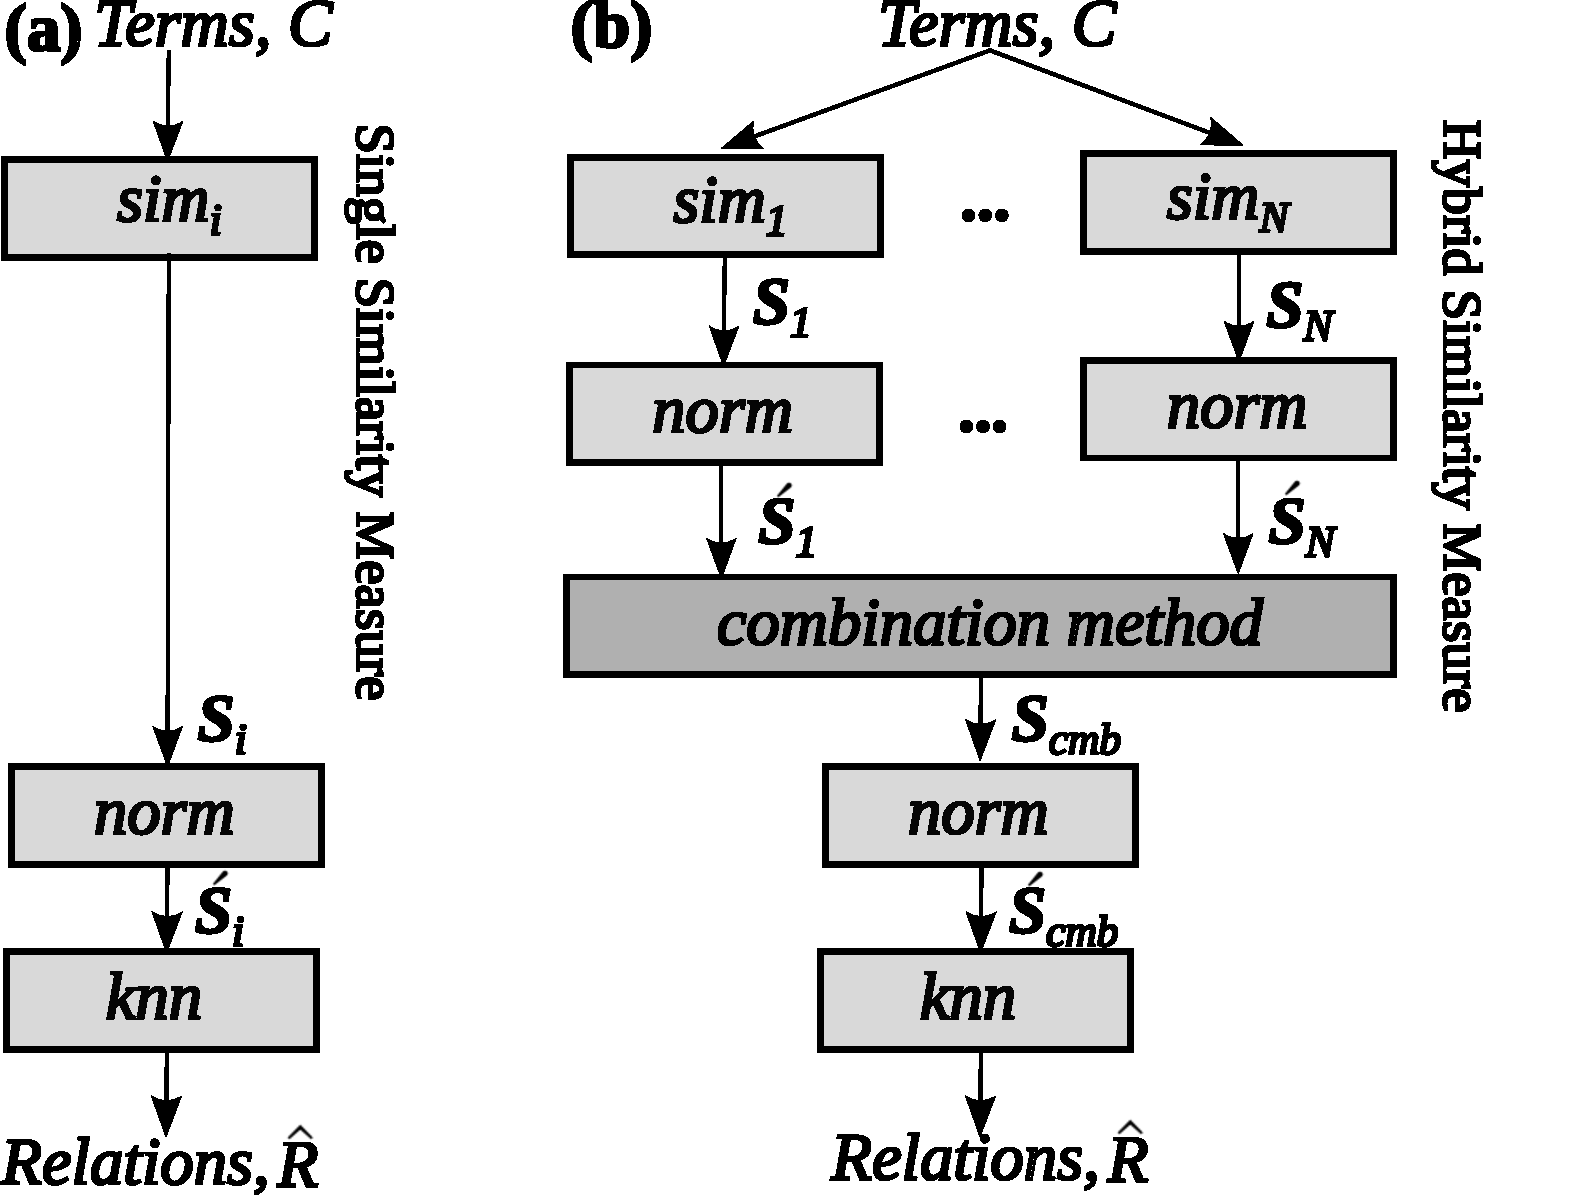
\includegraphics[width=0.65\textwidth]{./../figures/papers/4/src/figures/single-and-hybrid-2}
\caption{Система извлечения семантических отношений основанная на:
\begin{itemize}
\item \textbf{(a)} \textbf{отдельной} метрике;
\item \textbf{(b)} \textbf{гибридной} метрике. 
\end{itemize}}
\end{figure}
\end{frame}





\begin{frame}
\frametitle{16 признаков = 16 отдельных метрик}

    \begin{itemize}
    
    \item 5 метрик основанных на \textbf{семантических сетях}:
    \begin{enumerate}
      \item WuPalmer;
      \item Leacock and Chodorow;
      \item Resnik;
      \item Jiang and Conrath;
      \item Lin.
    \end{enumerate} 
    \item 3 метрики, основанные на \textbf{Веб корпусе} (NGD-Yahoo/Bing/Google);
        
    \item 5 метрики, основанные на \textbf{корпусе текстов}: 
    \begin{itemize}
      \item 2 дистрибутивных (BDA, SDA)
      \item 1 лексико-синтаксические шаблоны (PatternSim)
      \item 2 другие (LSA, NGD-Factiva)
    \end{itemize}
    
    \item 3 метрики, основанные на \textbf{определениях} 
    \begin{enumerate}
      \item ExtendedLesk;
      \item GlossVectors;
      \item DefVectors-WktWiki.
    \end{enumerate}
     
\end{itemize}

\end{frame}







\begin{frame}
\frametitle{Методы комбинирования без учителя}

\item $s_{ij}^k \in [0;1]$ -- попарное семантическое подобие слов $w_i$ и $w_j$, вычисленное с помощью $k$-й метрики $\mathbf{S}_k$.
 
\begin{block}{Mean}

Среднее между $K$ попарными подобиями слов:

$$s_{ij}^{cmb}= \frac{1}{K}\sum_{k=1,K} s_{ij}^k;$$

\end{block} 

\begin{block}{Mean-Nnz} 
Среднее между $K$ попарными подобиями слов больше нуля:

$$s_{ij}^{cmb}= \frac{1}{|k:s_{ij}^k >0,k=1,K|}\sum_{k=1,K} s_{ij}^k;$$

\end{block} 
\end{frame}







\begin{frame}
\frametitle{Методы комбинирования без учителя}


\begin{block}{Mean-Zscore}
Среднее между нормированными попарными подобиями слов (Z-score):

$$\mathbf{S}_{cmb} = \frac{1}{K} \sum_{k=1}^K \frac{\mathbf{S}_k -\mu_k}{\sigma_k};$$

где $\mu_k$ и $\sigma_k$ среднее и стандартное отклонение значений $k$-й метрики ($\mathbf{S}_k$).

\end{block} 

\begin{block}{Median}

Медиана между $K$ попарными подобиями слов:

$$s_{ij}^{cmb}= median(s_{ij}^1,\ldots,s_{ij}^K).$$

\end{block} 

\end{frame}






\begin{frame}
\frametitle{Методы комбинирования без учителя}

\begin{block}{Max}
Максимум между $K$ попарными подобиями слов:
$s_{ij}^{cmb}= max(s_{ij}^1,\ldots,s_{ij}^K);$
\end{block}

\begin{block}{RankFusion}
Среднее между рангами слов:
$$s_{ij}^{cmb}= \frac{1}{K}\sum_{k=1,K} r_{ij}^k.$$

где  $r^k_{ij}$ -- ранк, соответствующий значению попарного подобия $s^k_{ij}$.
\end{block}

%\item \textbf{RelationFusion} (Panchenko and Morozova, 2012).
%\end{enumerate}

\end{frame}






\begin{frame}
\frametitle{Методы комбинирования метрик подобия}

\begin{block}{RelationFusion}

Объединение отношений, извлеченных каждым методом. Отношения, извлеченные несколькими метриками, надежнее.

%\begin{itemize}
%\item Объединение отношений, извлеченных каждым методом
%\item Отношения, извлеченные несколькими метриками, надежнее. 
%\end{itemize}

\begin{algorithm}[H]
%\SetLine
\KwIn{Матрицы подобия, сгенерированные $K$ метриками $\{\mathbf{S}_1,\ldots,\mathbf{S}_K\}$, количество ближайших соседей $k$}
\KwOut{ Комбинированная матрица подобия, $\mathbf{S}_{cmb}$  }

\For{i=1,N}{$R_i \leftarrow knn(\mathbf{S}_i, k)$ \;
 $\mathbf{R}_i \leftarrow relation\_matrix(R_i)$}
$\mathbf{S}_{cmb} \leftarrow \frac{1}{N} \sum_{i=1}^N \mathbf{R}_i$ \;
\Return $\mathbf{S}_{cmb}$ \;
\label{rfusion}
\end{algorithm}

$$
relation\_matrix: r_{ij} = \left\{ 
  \begin{array}{l l}
    1 & \quad \text{if } \langle c_i, c_j \rangle \in R_k \\
    0 & \quad \text{else}\\
  \end{array} \right.
$$

\end{block}

\end{frame}






\begin{frame}
\frametitle{Методы комбинирования с учителем}

\begin{block}{Logit, Logit-L1, Logit-L2} 

\begin{itemize}
  \item  Бинарная \textbf{логистическая регрессия};

\item \textbf{Положительные обучающие примеры} -- синонимы, гиперонимы,
ко-гипонимы из BLESS/SN;
\item \textbf{Отрицательные обучающие примеры} -- случайные пары семантически
несвязных слов из BLESS/SN;

  \item Отношение $\langle c_i,t, c_j \rangle \in R$ представлено с помощью
  \textbf{вектора попарных близостей}: $\mathbf{x} = (s_{ij}^1,\ldots,s_{ij}^N),
  N=\overline{2,16}$;

\item Категория $y_{ij}$:
$$
y_{ij} = \left\{ 
  \begin{array}{l l}
    0 & \quad  \text{ если } \langle c_i,t, c_j \rangle \text{ случайное
    отношение}
    \\
    1 & \quad  \text{ иначе }\\
  \end{array} \right
  .
$$

\end{itemize}
\end{block}

\end{frame}










\begin{frame}
\frametitle{Методы комбинирования с учителем}

\begin{block}{Logit, Logit-L1, Logit-L2} 

\begin{itemize}

\item \textbf{Logit} максимизирует следующую функционал:

$$
L(\mathbf{w}) &=&  \max_{\mathbf{w}} \sum_{i=1}^N \ln s^{cmb}_{ij} + \sum_{i=1}^N\ln(1-s^{cmb}_{ij}) 
$$

\item \textbf{Использование модели} $(w_1,\ldots,w_K)$ для комбинирования: 
$$s^{cmb}_{ij} =  P(r_{ij}=1|s_{ij}^{1},\ldots,s_{ij}^{K}) = \frac{1}{1 + e^{-z}} \text{, где} $$

$$ z = \sum_{k=1}^K w_k s^k_{ij} + w_0.$$

  %\frac{1}{1 + e^{-w_0 + \sum_{k=1}^K w_k s^k_{ij}}}

\end{itemize}
\end{block}

\end{frame}




\begin{frame}
\frametitle{Модель комбинирования метрик}

\begin{figure}
\centering
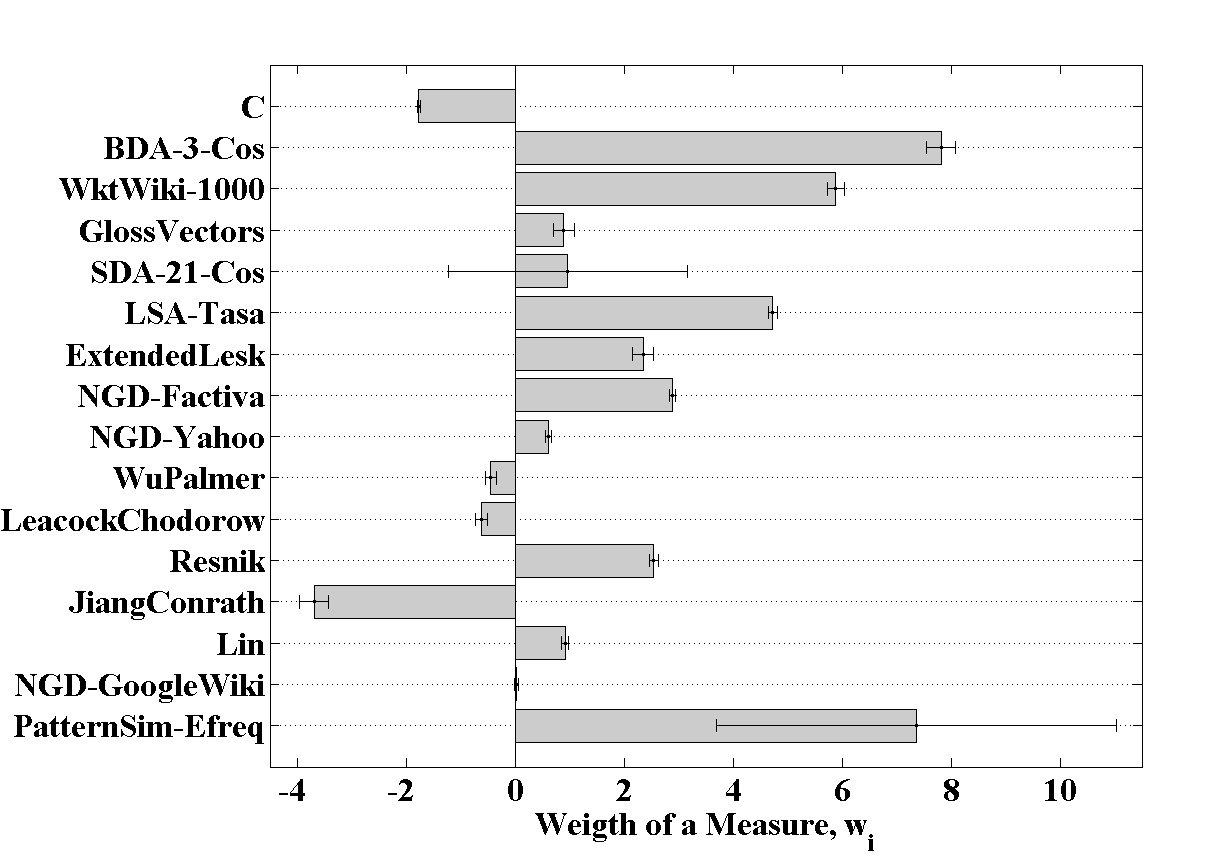
\includegraphics[width=0.7\textwidth]{../figures/chapter3/logit-e15-bless-errorbars}
\caption{ Weights of the similarity measures used by the hybrid measure Logit-E15. The weights were learnt on the BLESS dataset with 10-fold cross validation repeated 10 times. }
\end{figure}

\end{frame}





\begin{frame}
\frametitle{Методы комбинирования с учителем}

%\begin{block}{
\textbf{Машина Опорных Векторов (SVM), линейное ядро} 


\begin{columns}
  \begin{column}{0.5\textwidth}
\begin{figure}
\centering
\includegraphics[width=1.0\textwidth]{./../figures/svm}
%\caption{SVM: maximal margin hyperplane. }
\end{figure}
    
  \end{column}

  \begin{column}{0.5\textwidth}
\begin{itemize}
\item Веса $\mathbf{w}$ и опорные вектора $SV$: 

$$
\mathbf{w} = \sum_{x_i \in SV} \alpha_i y_i \mathbf{x}_i.  
$$

\item \textbf{Использование модели} 

$$
s_{ij}^{cmb} = \mathbf{w}^T\mathbf{x} + b = \sum_{k=1}^K w_i s_{ij}^k + b.
$$

\end{itemize}    
  \end{column}
\end{columns}

%\end{block}

\end{frame}




\begin{frame}
\frametitle{Машина Опорных Векторов (SVM), линейное ядро} 

\begin{itemize}

\item \textbf{Geometrical margin} is the distance to the closest data point: 
$$
\rho = \frac{\mathbf{w}^T\mathbf{x} - b}{||\mathbf{w}||}.
$$

%\item \textbf{Support vectors} -- are the closet points to the hyperplane

\item SVM maximizes the \textbf{margin} : $
\rho = \frac{\mathbf{w}^T\mathbf{x} - b}{||\mathbf{w}||} =  \frac{1}{||\mathbf{w}||}.
$

  
\item  Result -- a set of \textbf{support vectors}: $SV = \{\mathbf{x}_1,\ldots,\mathbf{x}_m\}$, where $y_i \in \{+1,-1\}$ is the label.



\item \textbf{Weight vector}: 
$ \mathbf{w} = \sum_{x_i \in SV} \alpha_i y_i \mathbf{x}_i.  $


\item $C$-SVM optimizes the following function:
\begin{eqnarray}
\min_{\mathbf{w}, \mathbf{\xi}, b} & \frac{1}{2} ||\mathbf{w}||^2 + C \sum_{i=1}^n \xi_i \\
\text{subject to} & y_i(\mathbf{w}^T\phi(x_i)) \geq 1 - \xi_i, \nonumber \\ 
& \xi_i \geq 0. \nonumber  
\end{eqnarray}


\item The function $\phi(\mathbf{x},\mathbf{x}')$ is called \textbf{kernel}.


\end{itemize}
\end{frame}







%%%%%%%%%%%%%%%%%%%%%%%%%%%%%%%%%%%%%%%%%%%%%%%%%
\begin{frame}
\frametitle{Какие из отдельных метрик следует комбинировать?}

\begin{block}{Количество возможных комбинаций}
 \begin{itemize}
 \item \alert{34}: $\sum_{m=2}^{34}C_{34}^m=\sum_{m=2}^{34}\frac{34!}{m!(34-m)!}= 2^{34}= 1.718 \cdot 10^{10}$
 \item \alert{16}: $\sum_{m=2}^{16}C_{16}^m=\sum_{m=2}^{16}\frac{16!}{m!(16-m)!}=65536$
 \end{itemize}
  \end{block}

\begin{itemize}

\item \textbf{Экспертный выбор}: \alert{5}, \alert{9} и \alert{15} метрик из 16
\item \textbf{Forward Stepwise Procedure}: \alert{7}, \alert{8}, \alert{8}, \alert{10} метрик из 16
\item Анализ коэффициентов \textbf{логистической регрессии}: \alert{12} из 16

%\begin{itemize}
 %\item \textbf{5} % = WN-Resnik, BDA-3-5000, SDA-21-100000,  Def-WktWiki-1000
 %\item \textbf{9} %= \textbf{Group4} + WN-WuPalmer, LSA-Tasa, Def-GlossVec., and Def-Ext.Les
 %\item \textbf{15} %= \textbf{Group8} + WN-LeacockChodorow, WN-Lin, WN-JiangConrath, NGD-Factiva, NGD-Yahoo, and NGD-GoogleWiki.
%\end{itemize}

\end{itemize}
\end{frame}
  


\begin{frame}
\frametitle{Результаты: базовые метрики, корреляция с суждениями субъектов}

\begin{figure}
\centering
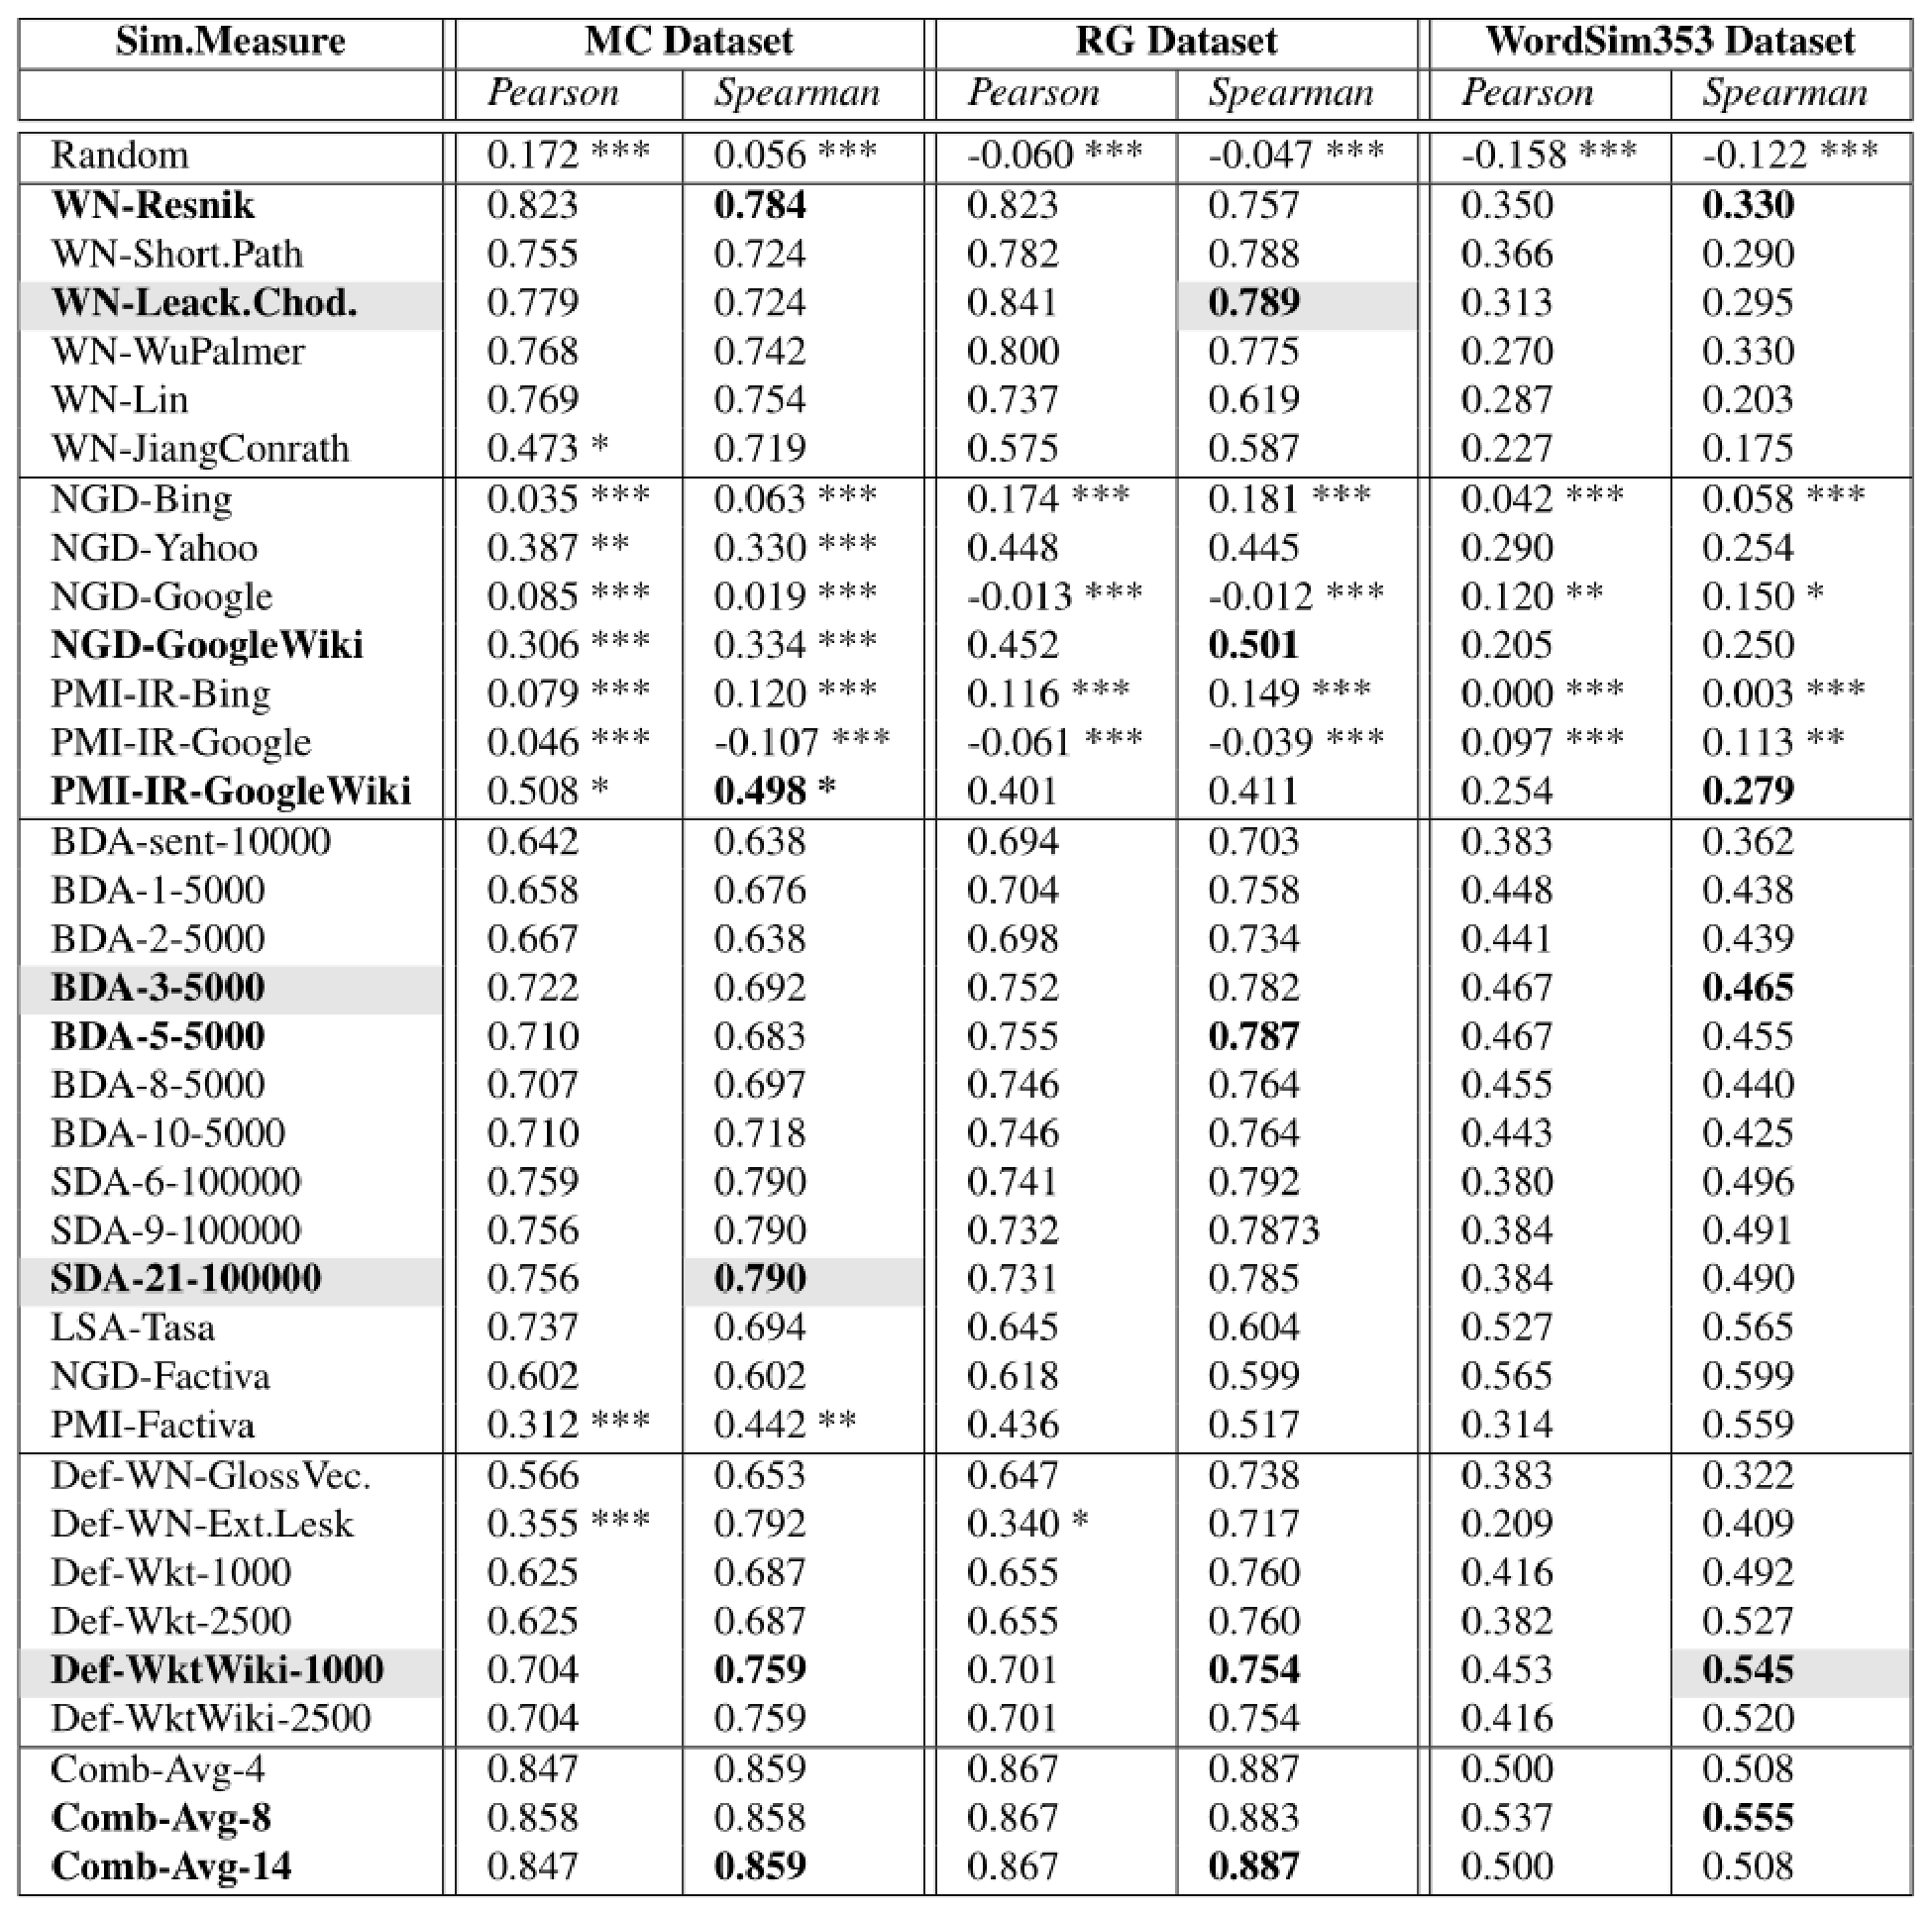
\includegraphics[width=0.52\textwidth]{figures/hj}
\caption{\footnotesize Pearson -- корреляция Пирсона, Spearman -- корреляция Спирмена.}
\end{figure}
    
\end{frame}





\begin{frame}
\frametitle{Результаты: базовые метрики, ранжирование отношний}

    \begin{figure}
    \centering
        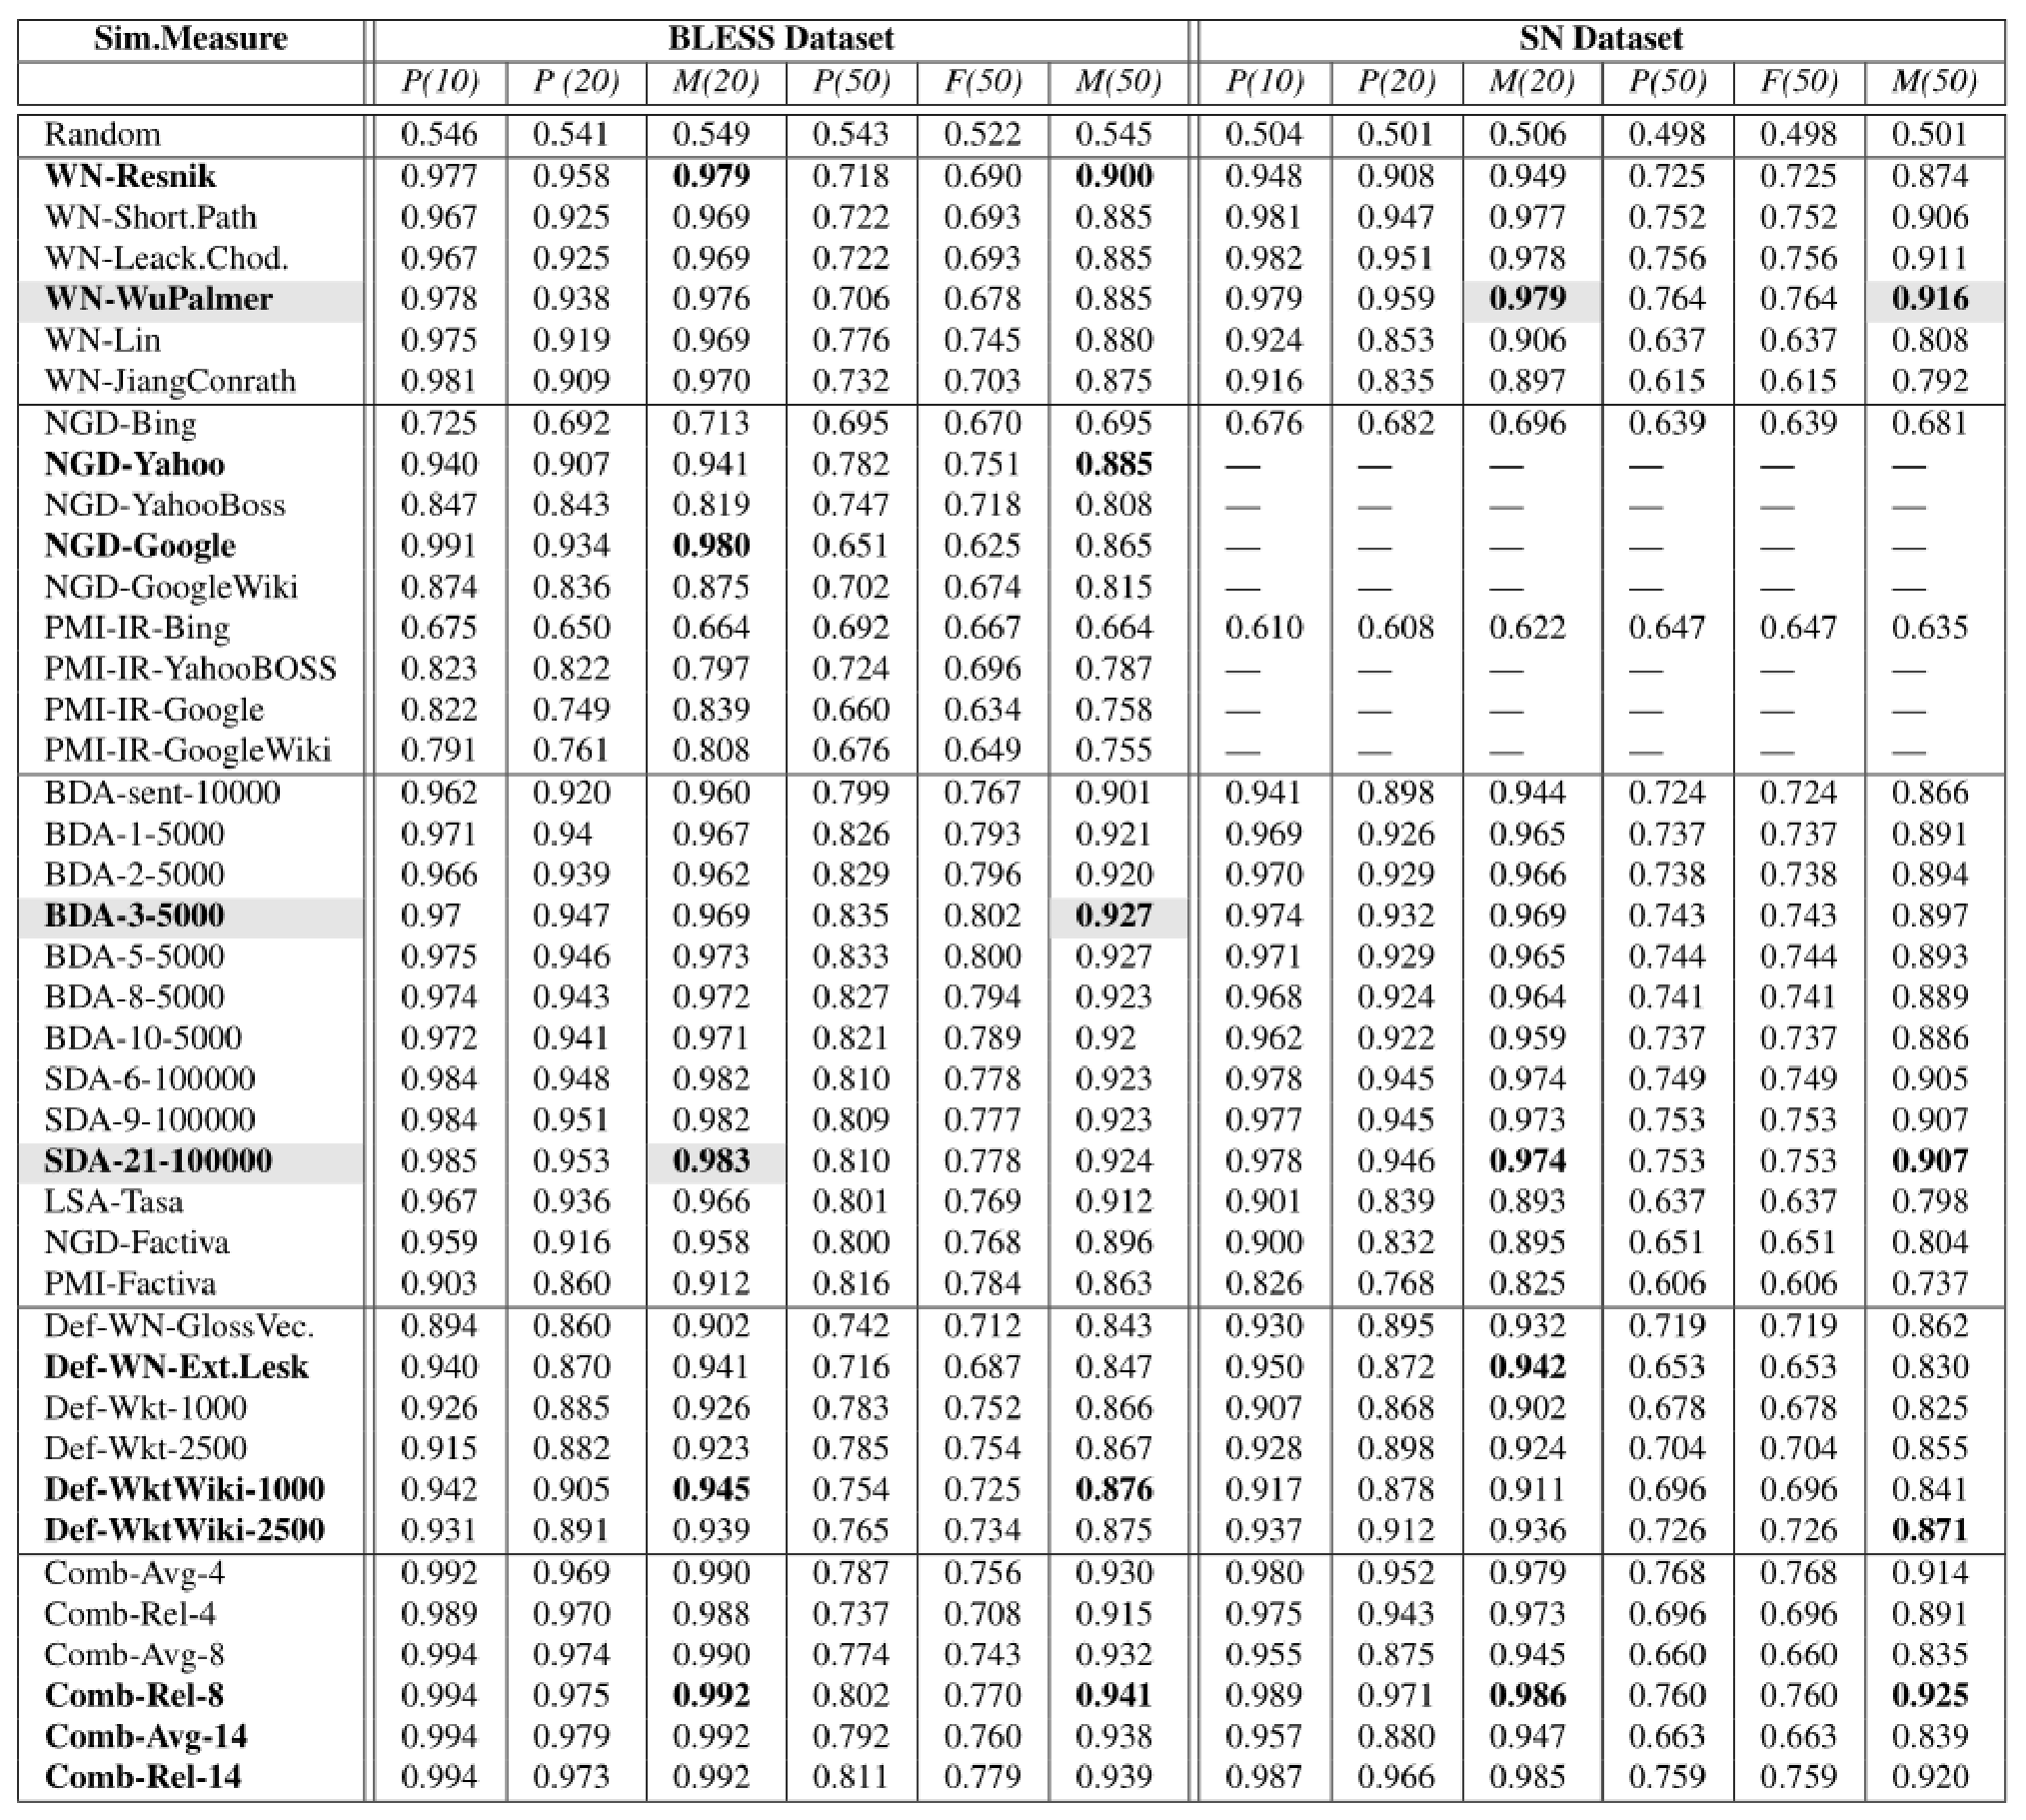
\includegraphics[width=0.7\textwidth]{figures/sr}
        %\caption{Здесь P -- точность, R -- полнота, F -- F1-мера, M -- MAP.}
        
\end{figure}
    
\end{frame}




\begin{frame}
\frametitle{Результаты: базовые метрики, ранжирование отношний}

    \begin{figure}
    \centering
        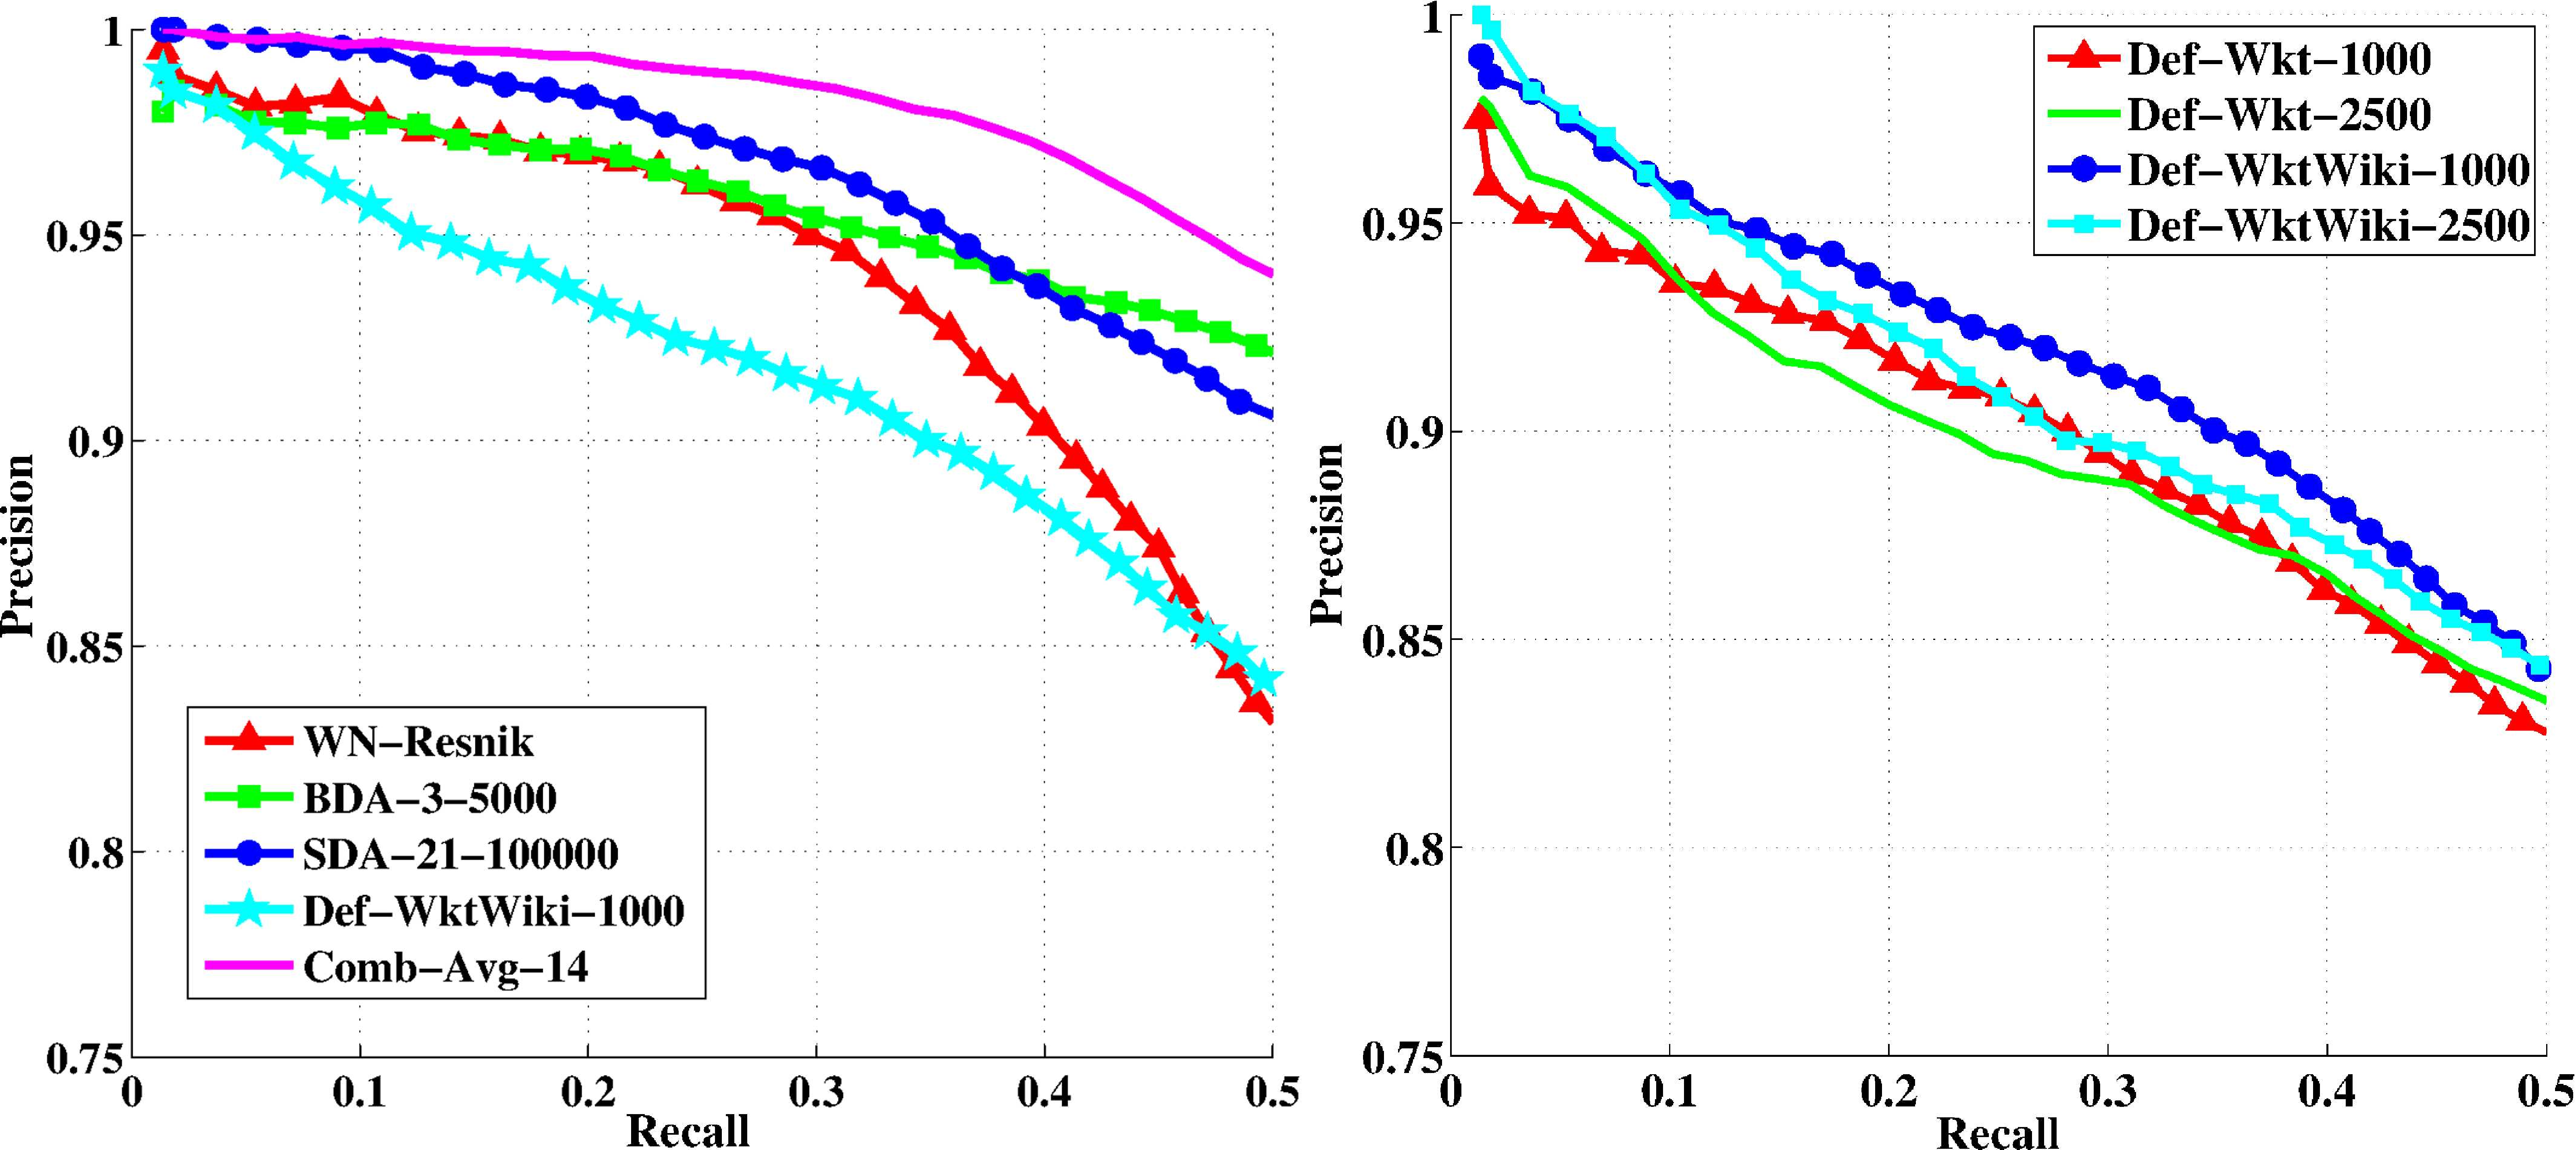
\includegraphics[width=1.0\textwidth]{../figures/pr-plots-2}
            \caption{Графики Точность-Полнота (слева) 4х лучших метрик основанных на корпусе, семантических сетях, определениях и метрика, основанная на среднем значении 14 метрик; (слева) метрики основанных на определениях Викисловаря и Википедии. }
\end{figure}
    
\end{frame}






%%%%%%%%%%%%%%%%%%%%%%%%%%%%%%%%%%%%%%%%%%%%%%%%%
\begin{frame}
\frametitle{Результаты: отдельные и комбинированные метрики }


    \begin{figure}
    \centering
        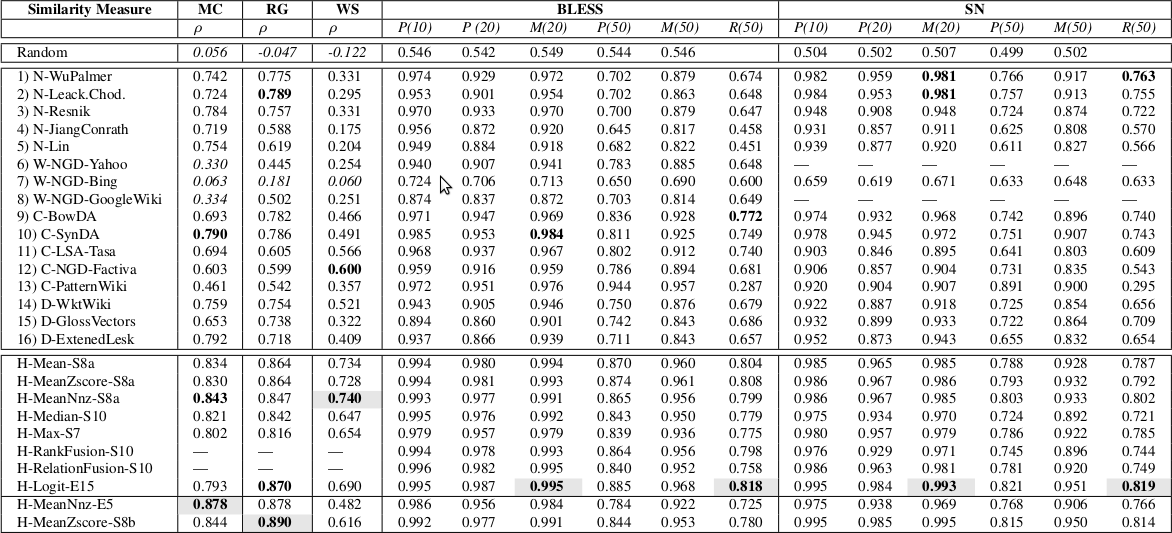
\includegraphics[width=1.0\textwidth]{figures/table-hybrid}
        \caption{
        \footnotesize
        Характеристики 16 отдельных и 8 комбинированных метрик. MC, RG, WordSim353 -- корреляция с суждениями человека. BLESS, SN -- точность извлечения семантических отношений. Наилучшие значения в группе (отдельные/комбинированные) обозначены полужирным шрифтом; наилучшие значения  обозначены серым цветом. }
\end{figure}
    
\end{frame}




\begin{frame}
\frametitle{Результаты: методы комбинирования с учителем}
\begin{figure}
\centering
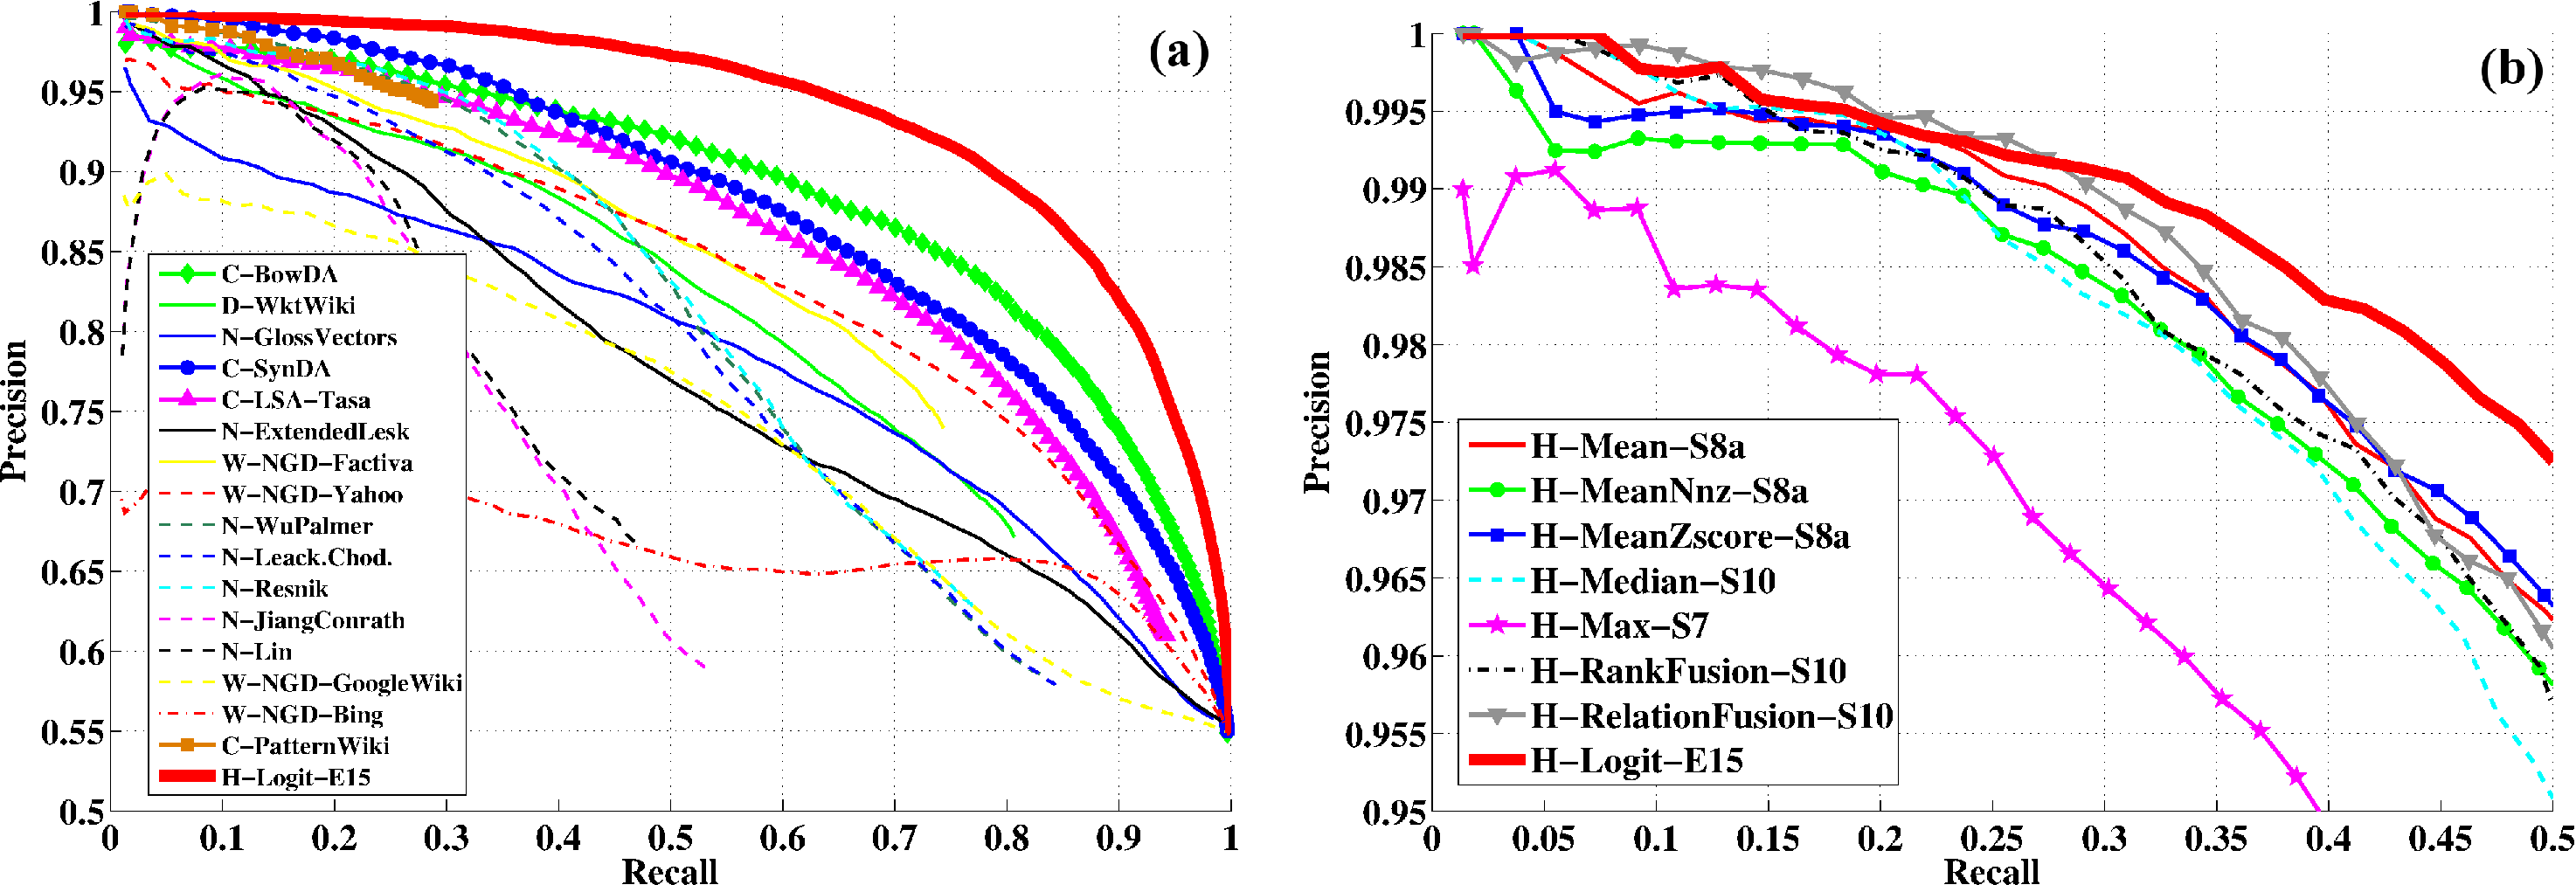
\includegraphics[width=1.0\textwidth]{figures/pr}
%\caption{

%}
\end{figure}

График Точность-Полнота вычисленный на коллекции BLESS:
\begin{itemize}
  \item \textbf{(a)} 16 отдельных метрик и гибридная метрика Logit-E15;
  \item \textbf{(b)} 8 гибридных метрик.
\end{itemize}

\end{frame}



\begin{frame}
\frametitle{Результаты: метод комбинирования с учителем Logit-E15}
\begin{figure}
\centering
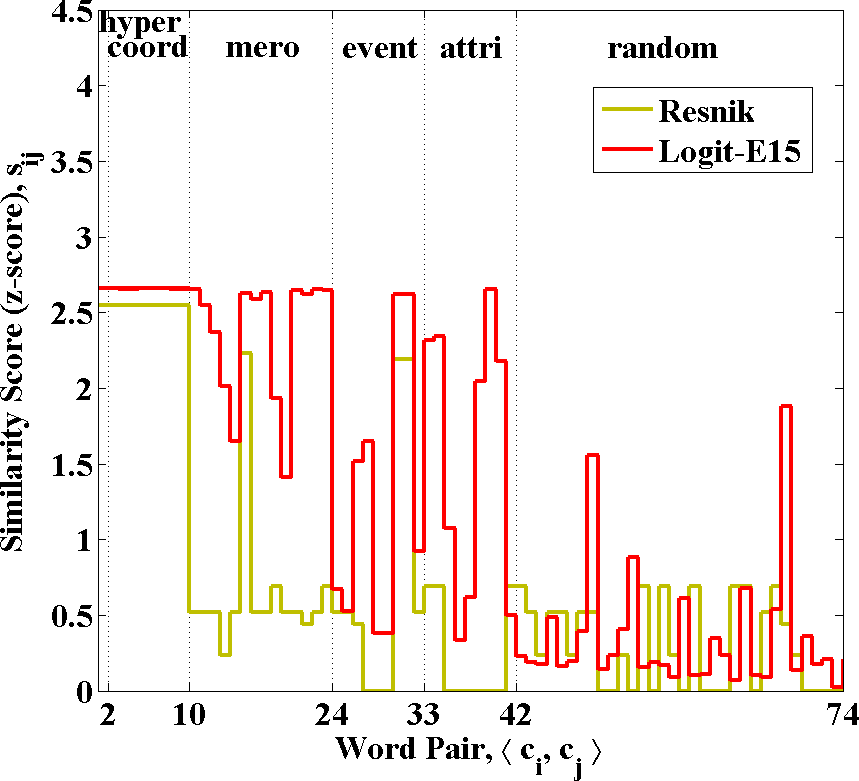
\includegraphics[width=0.30\textwidth]{figures/acacia-resnik} 
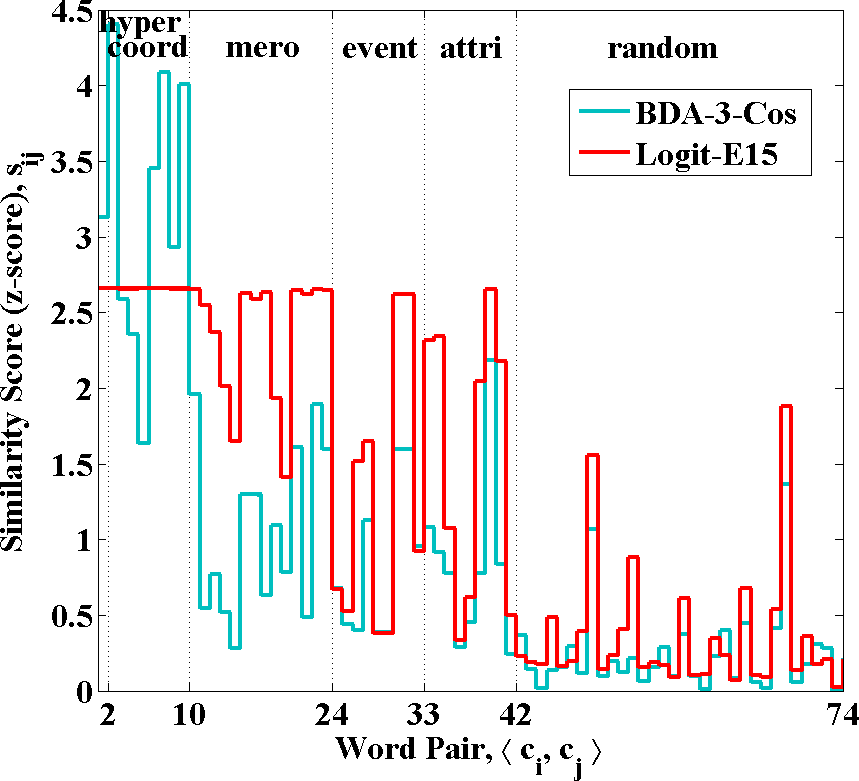
\includegraphics[width=0.30\textwidth]{figures/acacia-bda}
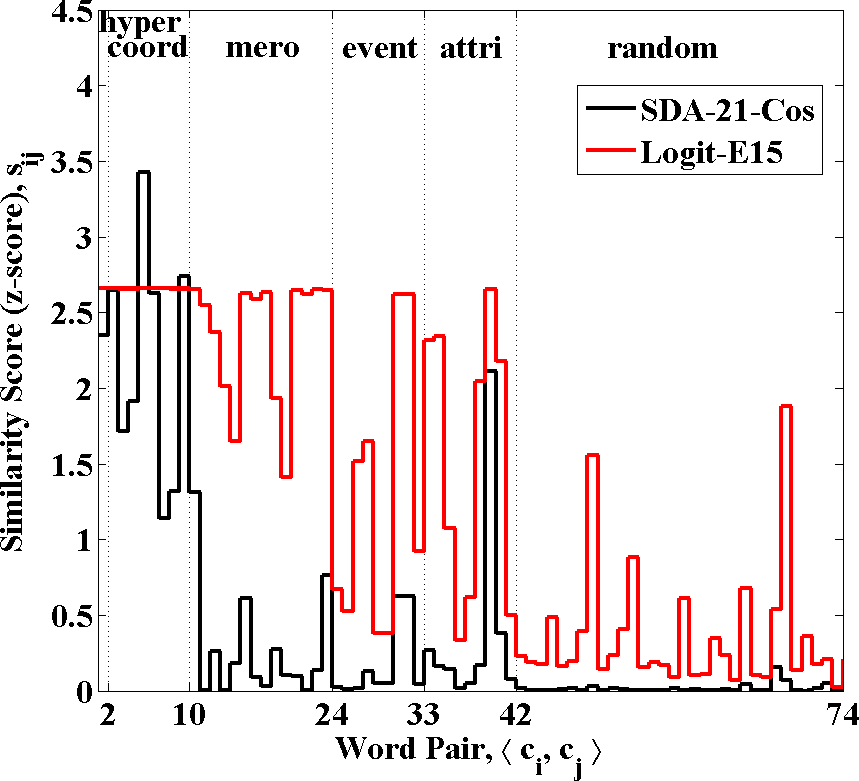
\includegraphics[width=0.30\textwidth]{figures/acacia-sda}

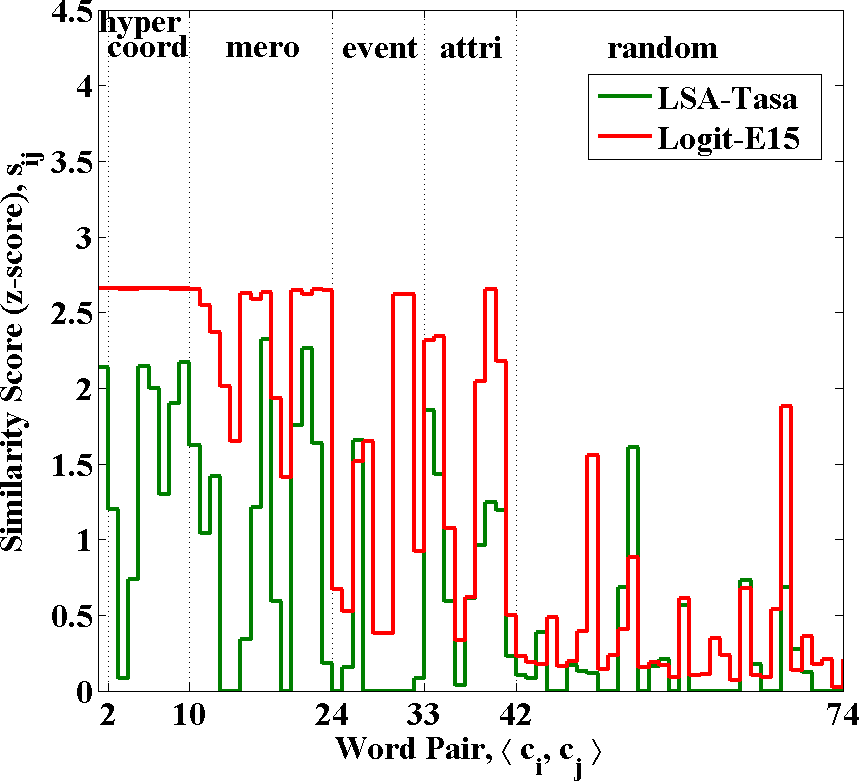
\includegraphics[width=0.30\textwidth]{figures/acacia-lsa}
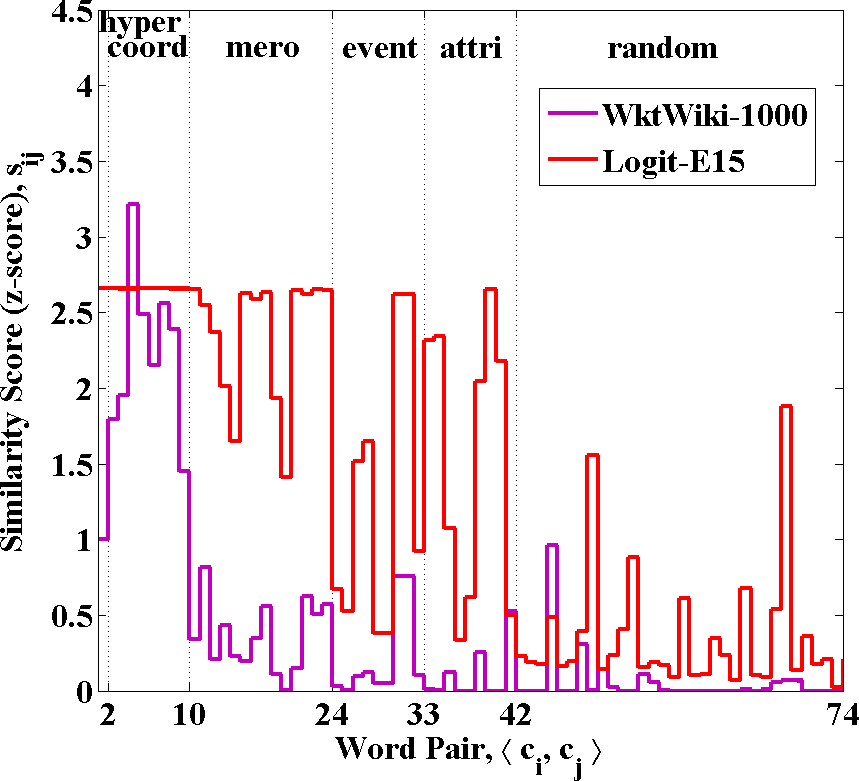
\includegraphics[width=0.30\textwidth]{figures/acacia-ww}
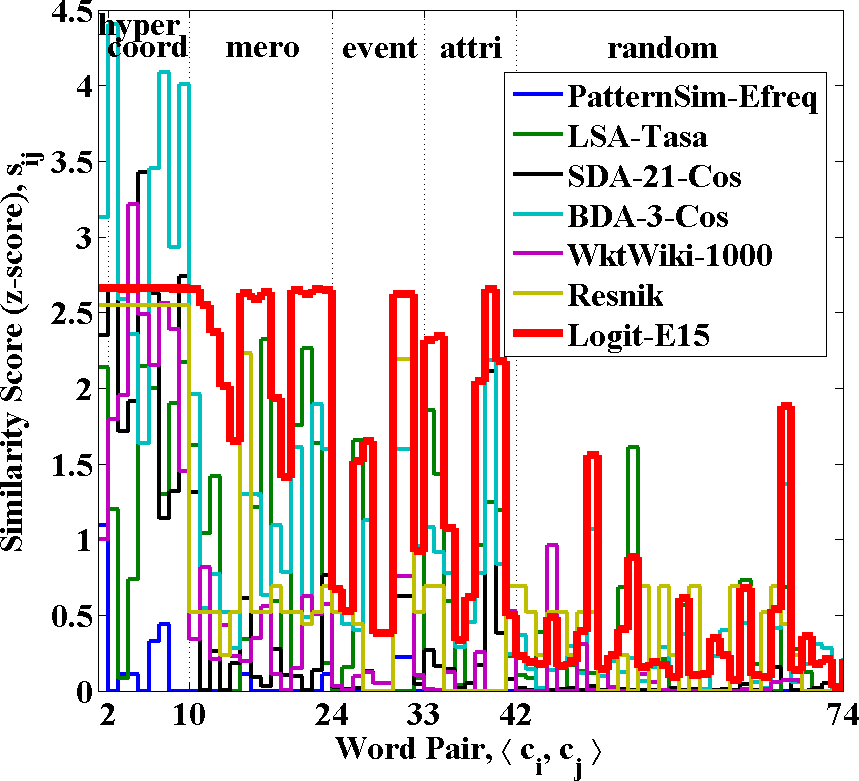
\includegraphics[width=0.30\textwidth]{figures/acacia}
\caption{ Значение подобия между 74 словами связанными со словом ``acacia''.
}
\label{fig:hybrid-complimentary-discussion}
\end{figure}

\end{frame}


\begin{frame}
\frametitle{Результаты: методы комбинирования с учителем}

    \begin{figure}
    \centering
        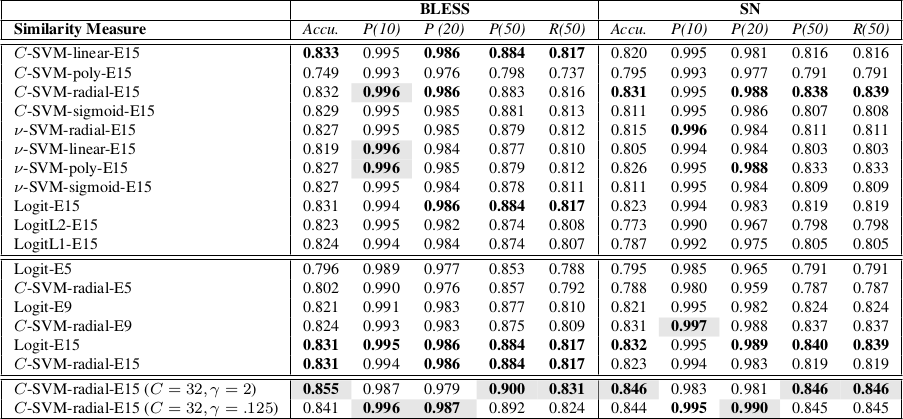
\includegraphics[width=1.0\textwidth]{figures/hybrid-table}
        
        %\caption{ Performance of the hybrid supervised semantic similarity measures. }
\end{figure}
\end{frame}


\begin{frame}
\frametitle{Результаты: методы комбинирования с учителем (продолжение)}
\begin{figure}
\centering
\includegraphics[height=0.4\textwidth]{./../figures/sn-accuracy}
\includegraphics[height=0.4\textwidth]{./../figures/bless-accuracy}
%
\includegraphics[height=0.025\textwidth]{./../figures/spacer}
%\includegraphics[height=0.36\textwidth]{./../figures/bless-precision10}
%\includegraphics[height=0.36\textwidth]{./../figures/bless-precision20}
%
\includegraphics[height=0.025\textwidth]{./../figures/spacer}
%\includegraphics[height=0.36\textwidth]{figures/bless-precision50}
%\includegraphics[height=0.36\textwidth]{figures/bless-recall50}     
     
\caption{ Оптимизация мета-параметров метрики C-SVM-radial-E15.  }
\label{fig:radial-optimization}
\end{figure}
\end{frame}


\section[Приложения]{Приложения метрик семантической близости}
\subsection{Поиск и визуализация семантически связанных слов}

  


\begin{frame}
\frametitle{Серелекс: результаты в виде списка и графа слов}

\begin{itemize}
\item \url{http://serelex.cental.be/}
\end{itemize}


\begin{figure}  
    \centering
    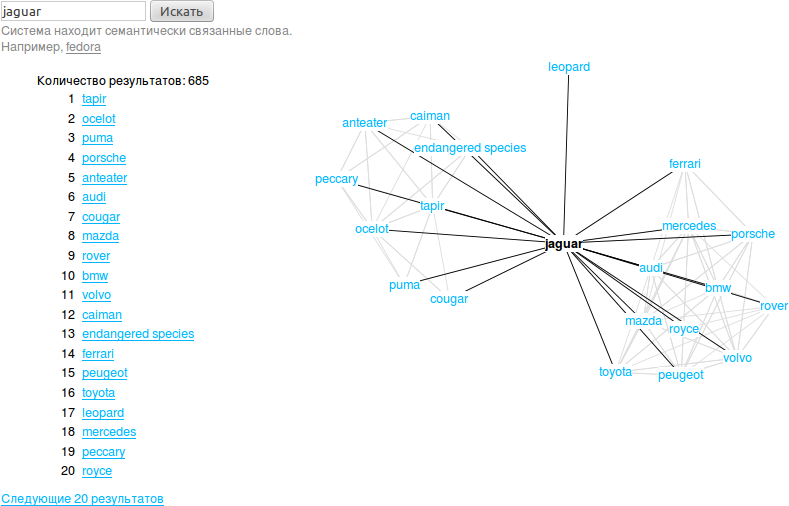
\includegraphics[width=0.9\textwidth]{jaguar}
\end{figure}

\end{frame}








\begin{frame}
\frametitle{Серелекс: результаты в виде графа слов}

\begin{figure}
\centering
\includegraphics[height=0.55\textwidth]{../figures/serelex-brussels}
\end{figure}

\end{frame}






\begin{frame}
\frametitle{Серелекс: результаты в виде графа слов}

\begin{figure}
\centering
%\includegraphics[height=0.55\textwidth]{../figures/serelex-brussels}
%
\includegraphics[width=1.0\textwidth]{figures/spacer}
\includegraphics[height=0.55\textwidth]{../figures/serelex-zurich}       
\end{figure}

\end{frame}






\begin{frame}
\frametitle{Серелекс: результаты в виде графа слов}

\begin{figure}
\centering
\includegraphics[width=0.6\textwidth]{../figures/serelex-big-graph-r}
\end{figure}

\end{frame}






\begin{frame}
\frametitle{Серелекс: результаты в виде множества изображений}

\includegraphics[width=1.0\textwidth]{./../figures/citroyen}

\end{frame}





\begin{frame}
\frametitle{Оценка качества работы системы Серелекс}

\begin{figure}
\center
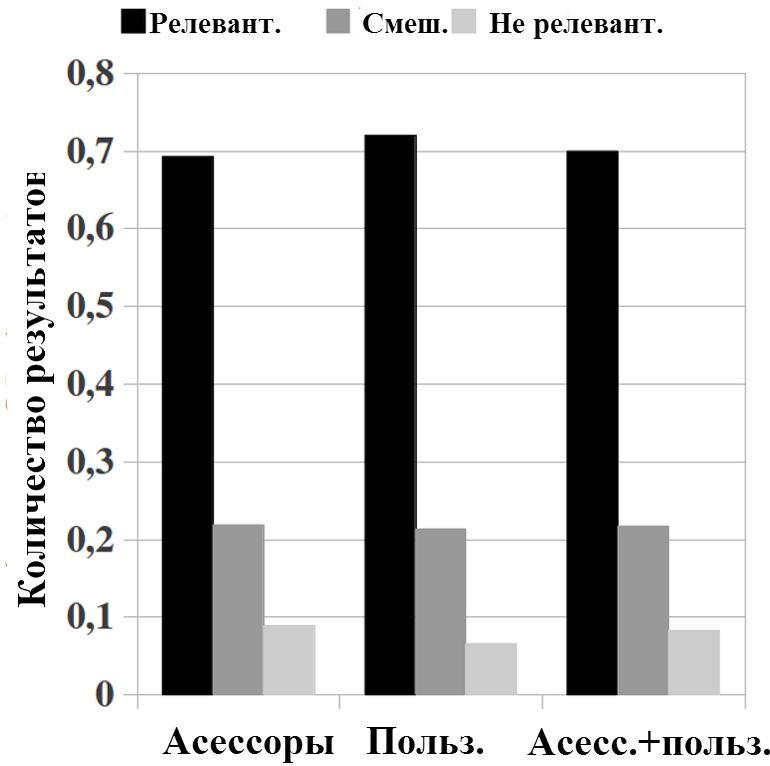
\includegraphics[width=0.5\textwidth]{serelex-eval}

\caption{Удовлетворенность пользователей первыми 20 результатами поиска для
594 запроса (23 ассесора и 109 пользователей).}
\end{figure}
\end{frame}




\begin{frame}
\frametitle{Оценка качества работы системы Серелекс}

\begin{figure}
\centering
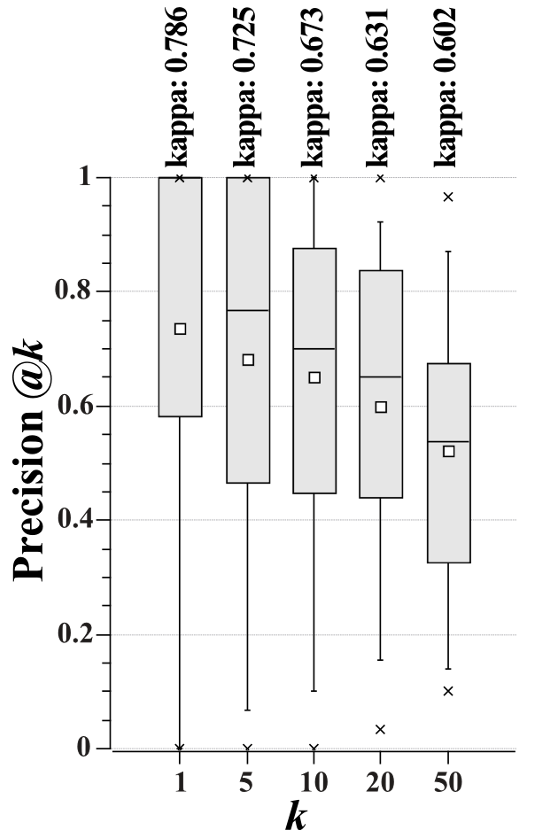
\includegraphics[width=0.4\textwidth]{figures/eval2-bc}     
\end{figure}

\end{frame}




\subsection{Классификация коротких текстов}

\begin{frame}[fragile]
\frametitle{iCop: классификация имен файлов}

\begin{figure}
\center
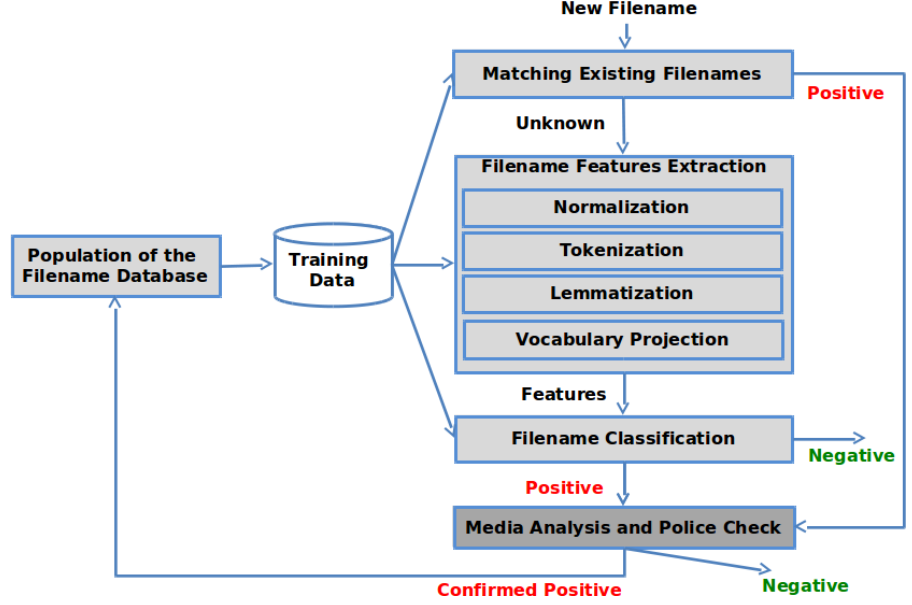
\includegraphics[width=0.7\textwidth]{./icop}
\caption{Структура системы.}
\end{figure}

\begin{itemize}
  \item Использование семантических отношений для расширения имени файла
  (Vocabulary Projection).
\end{itemize}


\end{frame}


\begin{frame}[fragile]
\frametitle{iCop: пример Vocabulary Projection}

\begin{figure}
\center
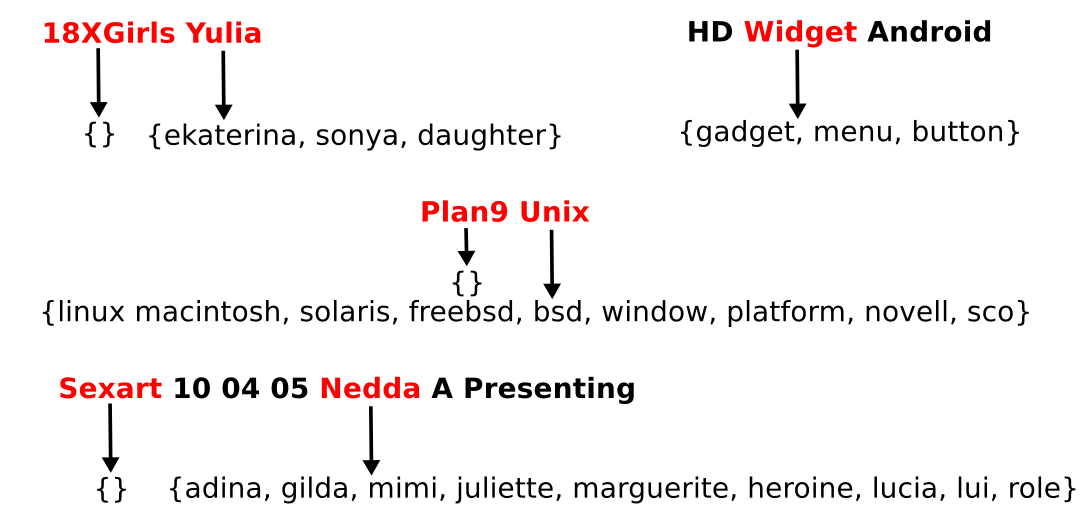
\includegraphics[width=0.9\textwidth]{./vp-ex}
\end{figure}



\end{frame}


\begin{frame}
\frametitle{Качество классификации}
\begin{table}
\tiny

%\footnotesize
\centering
\begin{tabular}{|l|l|l|l|}

\hline
\bf Обучающая выборка & \bf Тестовая выборка & \bf Accuracy  &
\textbf{Accuracy (voc. projection)} \\ \hline

Gallery (train) & Gallery  & 96.41 & \textbf{96.83} (+0.42) \\
PirateBay Title+Desc+Tags & PirateBay Title+Desc+Tags &  \textbf{98.92} &  98.86 (--0.06)\\
PirateBay Title+Tags & PirateBay Title+Tags & \textbf{97.73} & 97.63 (--0.10) \\
Gallery & PirateBay Title+Desc+Tags & 90.57 & \textbf{91.48} (+0.91) \\
\alert{Gallery}  & \alert{PirateBay Title+Tags}  & \alert{84.23} & \alert{\textbf{88.89}} \alert{(+4.66)} \\
PirateBay Title+Desc+Tags & Gallery  & 88.83 & \textbf{89.04} (+0.21) \\
PirateBay Title+Tags & Gallery & 91.16 & \textbf{91.30} (+0.14) \\
\hline

\end{tabular}
\caption{ Качество классификации с использованием C-SVM-linear c учетом
кросс-валидации.
}
\label{tbl:results2}

\end{table}
\end{frame}




\begin{frame}
\frametitle{Качество классификации}

\begin{figure}
\centering
\includegraphics[height=5.0cm]{../figures/papers/ecir-icop/figures/gallery2pirate} 
\caption{$C$-SVM-linear trained on the \textit{Gallery} dataset and tested on the \textit{PirateBay} dataset. }
\label{fig:gallery2pirate}
\end{figure}
\end{frame}




\begin{frame}
\frametitle{Анализ работы}

\begin{figure}
\centering
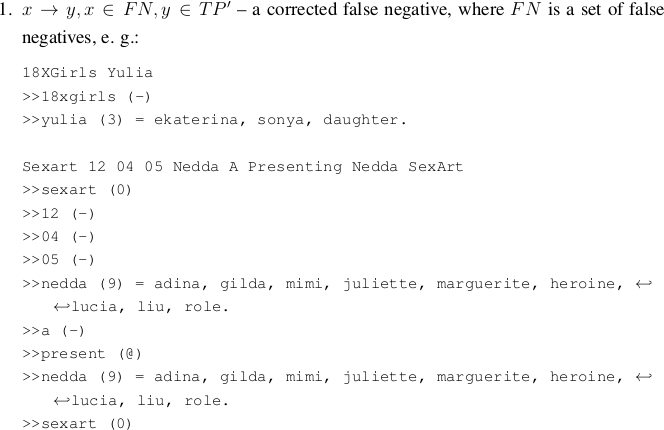
\includegraphics[width=0.9\textwidth]{figures/1}
\end{figure}
\end{frame}




\begin{frame}
\frametitle{Анализ работы}

\begin{figure}
\centering
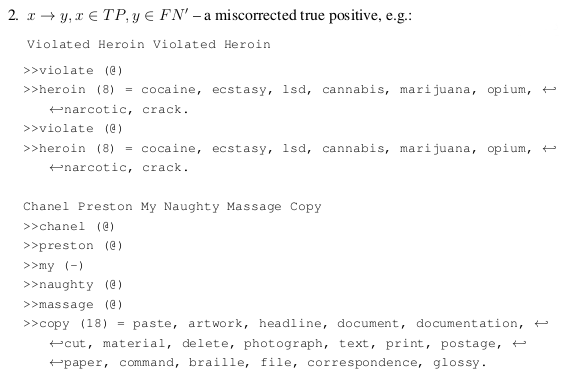
\includegraphics[width=0.9\textwidth]{figures/22}
\end{figure}
\end{frame}





\begin{frame}
\frametitle{Анализ работы}

\begin{figure}
\centering
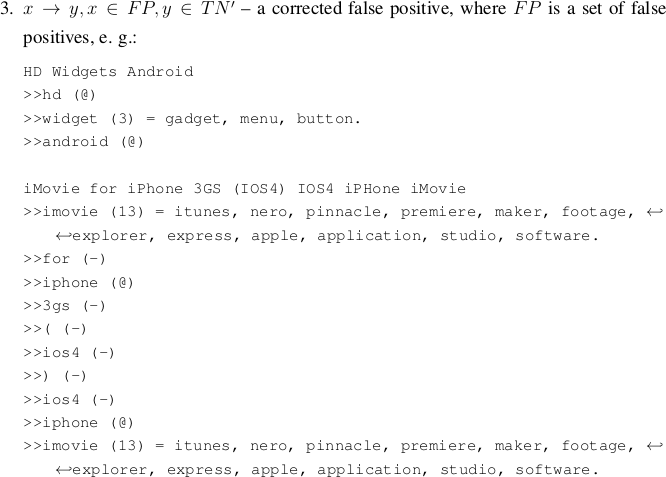
\includegraphics[width=0.9\textwidth]{figures/2}
\end{figure}
\end{frame}




\begin{frame}
\frametitle{Анализ работы}

\begin{figure}
\centering
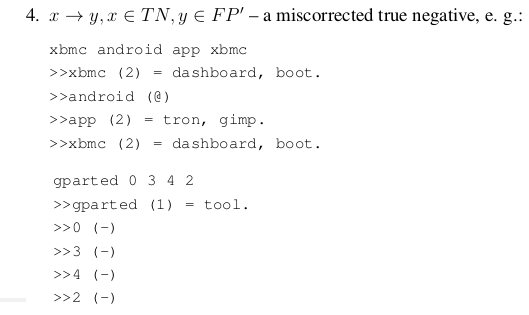
\includegraphics[width=0.9\textwidth]{figures/4}
\end{figure}
\end{frame}




%\section{Заключение}
%\subsection{}


%\begin{frame}
%\frametitle{The Key Contributions}

%### This dissertation explored several strategies to semantic relation extraction with similarity measures. 

% ### This work brings several contributions to the field of computational lexical semantics:

%\begin{enumerate}
%\item A corpus-based measure \textbf{SDA-MWE}: 
%\begin{itemize}
%\item performs comparably to the baselines;
%\item can deal with both single words and multiword expressions.
%\item was applied to automatic thesaurus construction.
%\end{itemize}

%\item A definition-based measure \textbf{DefVectors}:
%\begin{itemize}
%\item performs comparably to the baselines;
%\item operates on a small-scale set of definitions.
%\item an open source implemention.
%\end{itemize}
   
%\item A corpus-based measure \textbf{PatternSim}:
%\begin{itemize}
%\item performs comparably to the baseline measures;
%\item requires no semantic resources.
%\item an open source implemention.
%\end{itemize}

%\item A large-scale \textbf{comparative study} of the measures:
%\begin{itemize}
%\item comparison w.r.t. semantic relations provided by measures.
%\item evaluation scripts/datasets are available to the community.
%\end{itemize}


%\end{enumerate}

%\end{frame}

%\begin{frame}
%\frametitle{The Key Contributions (cont.)}

%\begin{enumerate}

%\setcounter{enumi}{4}



%\item Hybrid supervised semantic similarity measures \textbf{Logit-E15},
% \textbf{C-SVM-linear-E15}, \textbf{C-SVM-radial-E15}, etc.

%\begin{itemize}
 % \item based on the 5 types of resources;
 % \item outperforms baselines and other hybrid measures.

%\end{itemize}

%\item \textbf{Applications} which rely on the measure \textbf{PatternSim}:

%\begin{itemize}
%\item lexico-semantic search engine \textbf{Serelex};
%\begin{itemize}
%\item helps users discover similar words interactively;
%\item 70\% of users's satisfaction;
%\item an open source implementation.
%\end{itemize}

%\item Filename Categorization System system \textbf{iCOP}:
%\begin{itemize}
%\item categorizaton of file names;
%\item the measure refines accuracy of the baseline up to 5\%;
%\item an open source implementation. 
%\end{itemize}
% \end{itemize}

%\end{enumerate}

%\end{frame}



